\section{Client-server view (UML Component diagram)}\label{sec:client-server}
In Figure \ref{fig:cc-context}, we present a context diagram of the client-server view, detailing the external communication to and from the system. The entry points to the system are the (mostly automated) external version of raw data submission. The Customer Organisation and/or Social Secretary can submit Raw Data Batches via the specified protocols supported by the eDocs system.
The other entry point being the \ttt{UIfacade}, which is contacted by User Software for User Interface Actions, e.g. a management dashboard for the Customer Administrator (one or more per Organisation) to query for job statuses, or a log-in system for recipients to log in to the PDS.
The exit points of the system are more versatile. There is one closely related to the UI Actions, where parts of the system respond to queries by directly supplying information to the user sessions, which in turn are individual (dedicated) intermediaries for instances of the client software. This bypasses the \ttt{UIFacade} as a bottleneck.
The \ttt{SubmissionSubsystem} queries an \ttt{External Information Broker} when verifying the meta-data of Raw Data Batches and Entries as specified in \emph{UC3}.
The \ttt{BillingSubsystem} contacts the \ttt{Billing System} (external of the actual eDocs system) used by the eDocs Company periodically to bill users of eDocs.
The \ttt{CommunicationSubsystem} submits composed e-mails to an \ttt{External Email Provider} for delivery. This functionality is used for reporting errors in the system to the eDocs admin, various notifications to CO admins, delivery of documents etc.
There are two other external communication mechanisms for document delivery, namely the \ttt{Zoomit} service's \ttt{Document Delivery} interface and the \ttt{Print \& Postal Service}'s one. These are both directly used by the delivery subsystem, in contrast to document delivery by e-mail, which passes through the \ttt{CommunicationSubsystem}, as explained earlier.

\begin{figure}[!htp]
    \centering
    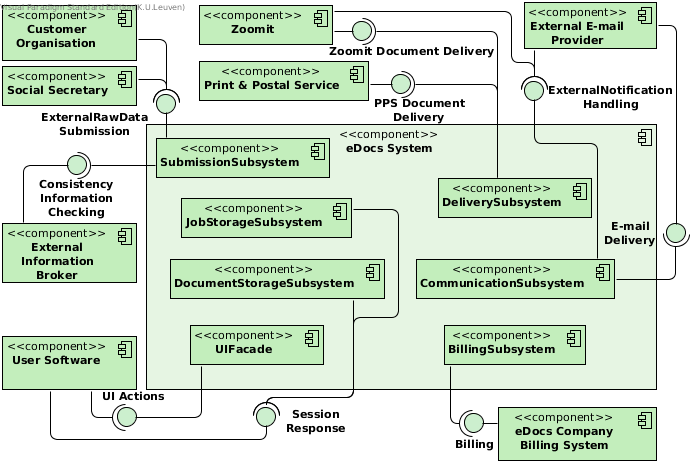
\includegraphics[width=\textwidth]{figures/Context Diagram 1.png}
    %\missingfigure[figwidth=0.8\textwidth]{Context diagram of the client-server view.}
    \caption{Context diagram for the client-server view.}\label{fig:cc-context}
\end{figure}

Figure \ref{fig:cs-primary} shows the primary component-and-connector diagram of the system. The presented overview divides the eDocs system into several subsystems, each with their dedicated functionalitie(s). The division are straightforward, and make for a less coupled system.\\
The \ttt{SubmissionSubsystem} accepts \ttt{Raw data batches} from an external user or via the \ttt{UIFacade}. It verifies these \ttt{Batches} and then registers them for generation in the \ttt{JobStorageSubsystem} and the \ttt{DocumentGenerationSubsystem}.\\
The \ttt{JobStorageSubsystem} \\
The \ttt{DocumentGenerationSubsystem} generates documents from submitted batches and applies scheduling based on deadlines of jobs. This generation consists of fetching the template for the document type of the document currently being generated, filling out the fields and any special steps befitting the document type (e.g. signing invoices). When finished, it hands the document to the \ttt{GeneratedDocumentHandler} for storage and delivery.\\
The \ttt{GeneratedDocumentHandler} \\
The \ttt{DocumentStorageSubsystem} is dedicated to the storage of documents. It has a database for \ttt{Personal Document Store} documents and a database for all documents; this means that the set of documents stored in the former is a subset of the set of documents stored in the latter. It also has an intermediary that makes constructing the \ttt{Personal Document Store} for newly registered Recipients more convenient on the one hand and an intermediary that contains a cache for documents to be stored in the \ttt{Personal Document Store} in case that database fails on the other.\\
The \ttt{DeliverySubsystem} \\
The \ttt{CommunicationSubsystem} handles outbound communication. There is a channel for notifications due to internal systems failure and a channel for all other communication. Due to the requirement that eDocs administrators be notified of any kind of failure within one minute (see \emph{Av1} and \emph{Av2}), the error channel can temporarily suppress the other communication to ensure that error notifications get to their destination on time.\\
The \ttt{UserManagementSubsystem} \\
The \ttt{BillingSubsystem} makes it possible to log any transaction consisting of document generation bills and document delivery bills, such that an invoice can be automatically sent to Customer Organizations for all activities performed on their behalf in a certain period. That period can be each month, each week or any other period length, whichever the financial department of eDocs deems most appropriate.\\
The \ttt{LookupSubsystem} processes requests for document lookups. It can handle requests where either a download link, a \ttt{JobID} or a search query is provided. In order to handle download links, there is a \ttt{LookupLinkCodec}, which can encode and decode downloads links (and also links specified to the \ttt{Personal Document Store}) and a \ttt{DownloadLinkCatalogue} where download links are stored for 30 days. If a Registered Recipient issues a query for the \ttt{Personal Document Store}, the \ttt{PDSLookupModule} handles that. To enable to system to throttle lookup requests (see \emph{P2}), there is a \ttt{LoadBalancer} which has to explicitly approve each lookup before it can be executed.\\
The \ttt{UIFacade} \\

\begin{figure}[!htp]
    \centering
    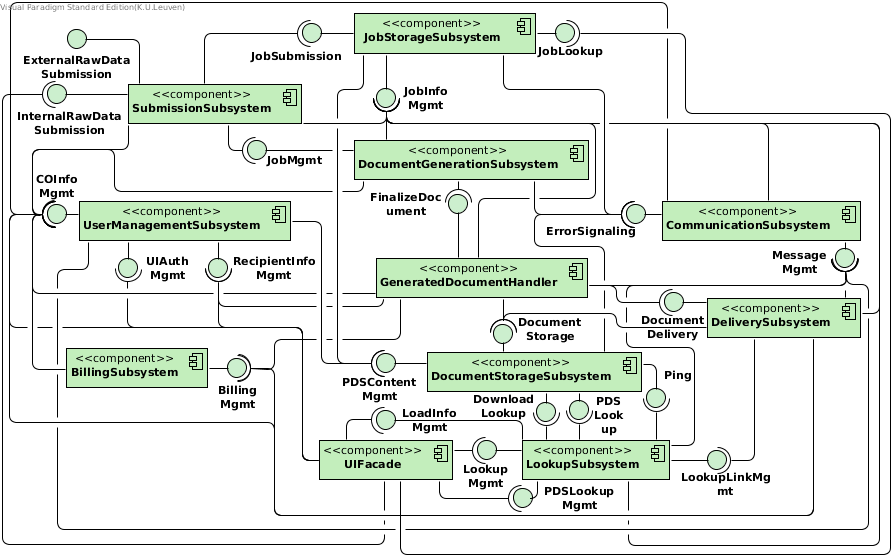
\includegraphics[width=\textwidth]{figures/Subsystem Diagram.png}
    %\missingfigure[figwidth=0.8\textwidth]{Primary diagram of the client-server view.}
    \caption{Primary component-and-connector view of the proposed architecture.}\label{fig:cs-primary}
\end{figure}

\subsection{Main architectural decisions}
Discuss your architectural decisions for the most important requirements in
more detail using the components of the client-server view.
Pay attention to the solutions that you employed and the alternatives that you
considered.
The explanation here must be self-contained and complete.
Imagine you had to describe how the architecture supports the core
functionality to someone that is looking at the client-server view only.
Hide unnecessary details (these should be shown in the decomposition view).

\subsubsection{Av1a and Av2a: notification of the eDocs Administrator}
Describe the design choices related to \emph{ReqX} together with the rationale
of why these choices where made.

\subsubsection*{Alternatives considered}
\paragraph{Alternative(s) for choice 1} Explain what alternative(s) you
considered for this design choice and why they where not selected.

\subsubsection{Av1b: storing the status of an individual job}
Describe the design choices related to \emph{ReqX} together with the rationale
of why these choices where made.

\subsubsection*{Alternatives considered}
\paragraph{Alternative(s) for choice 1} Explain what alternative(s) you
considered for this design choice and why they where not selected.

\subsubsection{Av2b: temporary storage of Personal Document Store documents}
Describe the design choices related to \emph{ReqX} together with the rationale
of why these choices where made.

\subsubsection*{Alternatives considered}
\paragraph{Alternative(s) for choice 1} Explain what alternative(s) you
considered for this design choice and why they where not selected.

\subsubsection{Av3: Zoomit failure}
Describe the design choices related to \emph{ReqX} together with the rationale
of why these choices where made.

\subsubsection*{Alternatives considered}
\paragraph{Alternative(s) for choice 1} Explain what alternative(s) you
considered for this design choice and why they where not selected.

\subsubsection{P2: document lookups}
Describe the design choices related to \emph{ReqX} together with the rationale
of why these choices where made.

\subsubsection*{Alternatives considered}
\paragraph{Alternative(s) for choice 1} Explain what alternative(s) you
considered for this design choice and why they where not selected.

\subsubsection{P3: status overview for Customer Administrators}
Describe the design choices related to \emph{ReqX} together with the rationale
of why these choices where made.

\subsubsection*{Alternatives considered}
\paragraph{Alternative(s) for choice 1} Explain what alternative(s) you
considered for this design choice and why they where not selected.

\subsubsection{M1: New type of document - bank statements}
Describe the design choices related to \emph{ReqX} together with the rationale
of why these choices where made.

\subsubsection*{Alternatives considered}
\paragraph{Alternative(s) for choice 1} Explain what alternative(s) you
considered for this design choice and why they where not selected.

\subsubsection{M2: Multiple print \& postal services}
Describe the design choices related to \emph{ReqX} together with the rationale
of why these choices where made.

\subsubsection*{Alternatives considered}
\paragraph{Alternative(s) for choice 1} Explain what alternative(s) you
considered for this design choice and why they where not selected.

\subsubsection{M3: Dynamic selection of the cheapest of print \& postal services}
Describe the design choices related to \emph{ReqX} together with the rationale
of why these choices where made.

\subsubsection*{Alternatives considered}
\paragraph{Alternative(s) for choice 1} Explain what alternative(s) you
considered for this design choice and why they where not selected.
